\documentclass[a4paper,oneside,10pt]{article}

\usepackage{subfiles}          % single chapter compiling

\usepackage[T1]{fontenc}       % font encoding
\usepackage[utf8]{inputenc}    % input encoding
\usepackage{lmodern}           % correct fonts to make pdf searchable

 % change page layout
\usepackage[left=2.5cm,right=2.5cm,bottom=3cm,top=3.5cm,a4paper]{geometry}

\usepackage{fancyhdr}          % fancy (=custom) headers/footers
\fancyhf{}                     % remove old headers
\pagestyle{fancy}              % enable fancy page style
% redefine section headersto avoid capitalization
\renewcommand{\sectionmark}[1]{\markboth{#1}{}}
\fancyhead[C]{\leftmark}       % section name above ../chapters
\fancyfoot[C]{\thepage}        % page number in the footer

\usepackage{amsmath, amssymb}  % math package

\usepackage{hyperref}          % clickable references
\hypersetup{hidelinks}         % links look like normal text
\usepackage{bookmark}          % to insert custom bookmarks

\usepackage{graphicx}          % graphics
\usepackage{subcaption}        % multiple figures
\usepackage{multirow}          % for rowspanning table entries
\usepackage{etoolbox}          % for conditional includes
\usepackage{pdfpages}          % to include exercise sheets
\usepackage{array}             % better tables
\usepackage{makecell}          % better tables
%\newcolumntype{x}[1]{>{\centering\arraybackslash}p{#1}}
\usepackage{tabularx}
\usepackage{slashbox}
\usepackage{xcolor,colortbl}
\usepackage{makeidx}           % make a word index
\makeindex  
\usepackage[totoc]{idxlayout}  % add index to table of contents

\usepackage{tikz}              % diagrams
\usetikzlibrary{trees}         % tree diagrams
\usetikzlibrary{patterns}      % patterns to fill areas below graphs

\usepackage{pgfplots}          % complex functions
\pgfplotsset{compat=1.8}
% gauss(\mu, \sigma)
% normal gauss function
\pgfmathdeclarefunction{gauss}{2}{\pgfmathparse{1/(#2*sqrt(2*pi))*exp(-((x-#1)^2)/(2*#2^2))}}
% Gauss(\mu, \sigma)
% error function, numerical approximation of the gauss integration
\pgfmathdeclarefunction{Gauss}{2}{\pgfmathparse{( 1 /(1 + exp(-0.07056*((x-#1)/#2)^3 - 1.5976*(x-#1)/#2) )}}

% betaDist(\alpha, \beta)
\pgfkeys{/pgf/fpu} % allows calculations with high exponents, still better pre-calculate results for alpha/beta > 250
\pgfmathdeclarefunction{betaDist}{2}{\pgfmathparse{( x^(#1-1)*(1-x)^(#2-1) ) / ( ( (#1-1)! * (#2-1)! ) / ( ( #1 + #2 - 1 )! ) )}}
\edef\tmp{\pgfmathresult}
\pgfkeys{/pgf/fpu=false}

% Create diagonal seperated cell
%\newcommand\diag[4]{%
  %\multicolumn{1}{p{#2}}{\hskip-\tabcolsep
  %$\vcenter{\begin{tikzpicture}[baseline=0,anchor=south west,inner sep=#1]
  %\path[use as bounding box] (0,0) rectangle (#2+2\tabcolsep,\baselineskip);
  %\node[minimum width={#2+2\tabcolsep-\pgflinewidth},
        %minimum  height=\baselineskip+\extrarowheight-\pgflinewidth] (box) {};
  %\draw[line cap=round] (box.north west) -- (box.south east);
  %\node[anchor=south west] at (box.south west) {#3};
  %\node[anchor=north east] at (box.north east) {#4};
 %\end{tikzpicture}}$\hskip-\tabcolsep}}


% START fill area below graph
\tikzset{
  hatch distance/.store in=\hatchdistance,
  hatch distance=10pt,
  hatch thickness/.store in=\hatchthickness,
  hatch thickness=2pt
}
\makeatletter
\pgfdeclarepatternformonly[\hatchdistance,\hatchthickness]{flexible hatch}
{\pgfqpoint{0pt}{0pt}}
{\pgfqpoint{\hatchdistance}{\hatchdistance}}
{\pgfpoint{\hatchdistance-1pt}{\hatchdistance-1pt}}%
{
  \pgfsetcolor{\tikz@pattern@color}
  \pgfsetlinewidth{\hatchthickness}
  \pgfpathmoveto{\pgfqpoint{0pt}{0pt}}
  \pgfpathlineto{\pgfqpoint{\hatchdistance}{\hatchdistance}}
  \pgfusepath{stroke}
}
% END fill area below graph

\usepackage{mcode} % matlab source

\usepackage{eurosym}           % euro symbol
\DeclareRobustCommand{\officialeuro}{
  \ifmmode\expandafter\text\fi
  {\fontencoding{U}\fontfamily{eurosym}\selectfont e}} % euro symbol in math


\usepackage{wrapfig}           % package used for sidenotes
\newcommand{\sidenote}[2][.3]{ % sidenotes for texts
  \begin{wrapfigure}{o}{#1\textwidth}
    \vspace{-1.3em}
    \textbf{Note: }\textit{#2}
    \vspace{-1.3em}
  \end{wrapfigure}}


% Toggles for document layout
\newtoggle{exercises}   % toggle for exercise sheets
\newtoggle{solutions}   % toggle for sheet solutions
\newtoggle{showdates}   % toggle for dates in headlines
% use \toggletrue{} and \togglefalse{} to set them 

\toggletrue{exercises}
%\togglefalse{exercises} 

\toggletrue{solutions} 
%\togglefalse{solutions} 

\toggletrue{showdates}
%\togglefalse{showdates}

\setlength\parindent{0pt} % no indentation

% \est{q} creates the estimation for a variable (i.e. places ^ over it)
\newcommand{\est}[1]{\expandafter\hat#1}




\begin{document}

% title, no headings etc.
\pagestyle{empty}
\subfile{../chapters/titlepage.tex}
\clearpage

% bookmark for table of contents
\belowpdfbookmark{\contentsname}{Contents}
% table of contents and new page
\tableofcontents
\clearpage

% from now on headings etc.
\pagestyle{fancy}


% maybe one day we want to include a preface
%\subfile{../chapters/preface.tex}
%\clearpage


% Probability Refresher I
\subfile{../chapters/2014-04-22.tex}
\clearpage

% Practice: Probability Refresher I
\iftoggle{exercises}{
  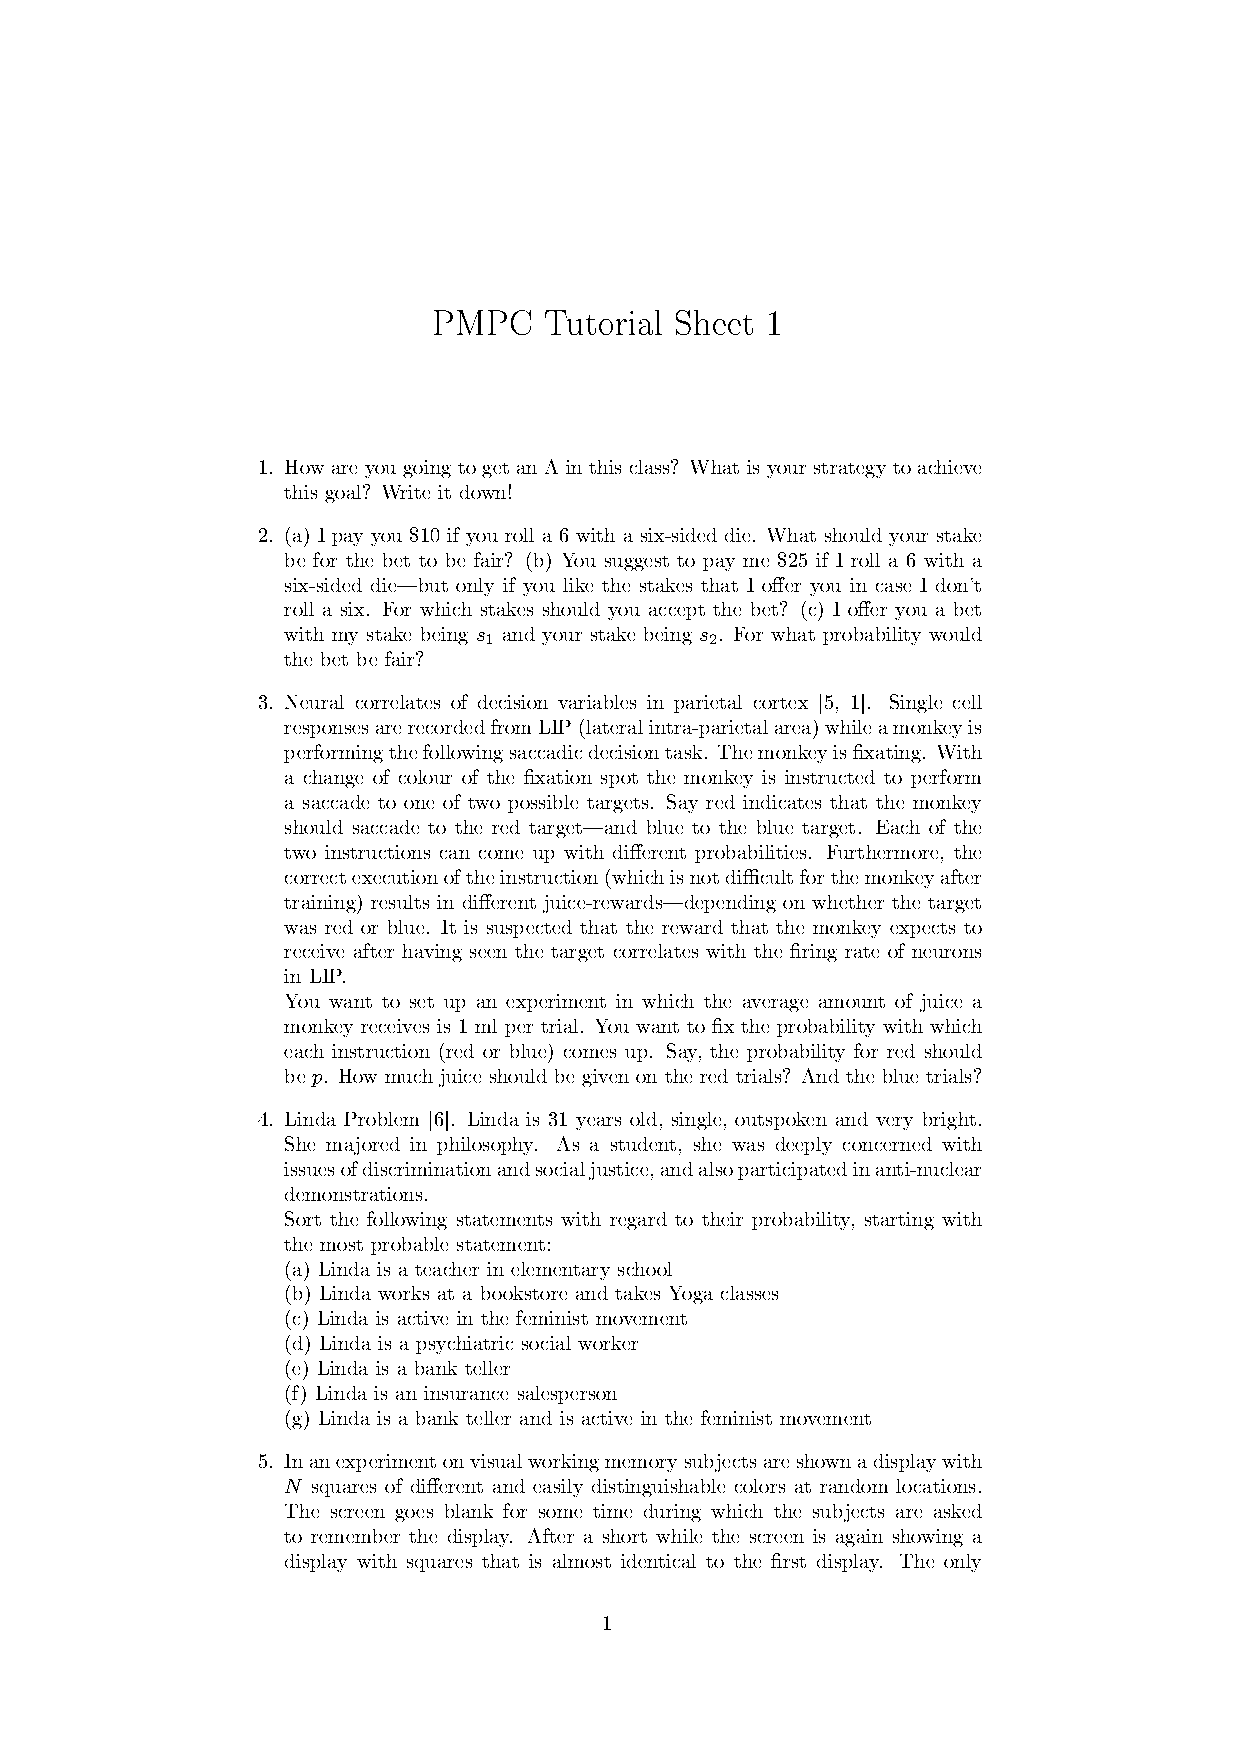
\includepdf[pages={-},
      addtotoc={1,section,1,Tutorial Sheet 1: Probability Refresher I,exsheet1},
      viewport=100 50 550 700,
      scale=0.75,
      pagecommand=\thispagestyle{plain}
      ]{../exercises/Exercises01.pdf}
}{}
\iftoggle{solutions}{
  \subfile{../chapters/2014-04-28.tex}
  \clearpage
}{}

% Probability Refresher II
\subfile{../chapters/2014-04-25.tex}
\clearpage

% Practice: Probability Refresher II
\iftoggle{exercises}{
  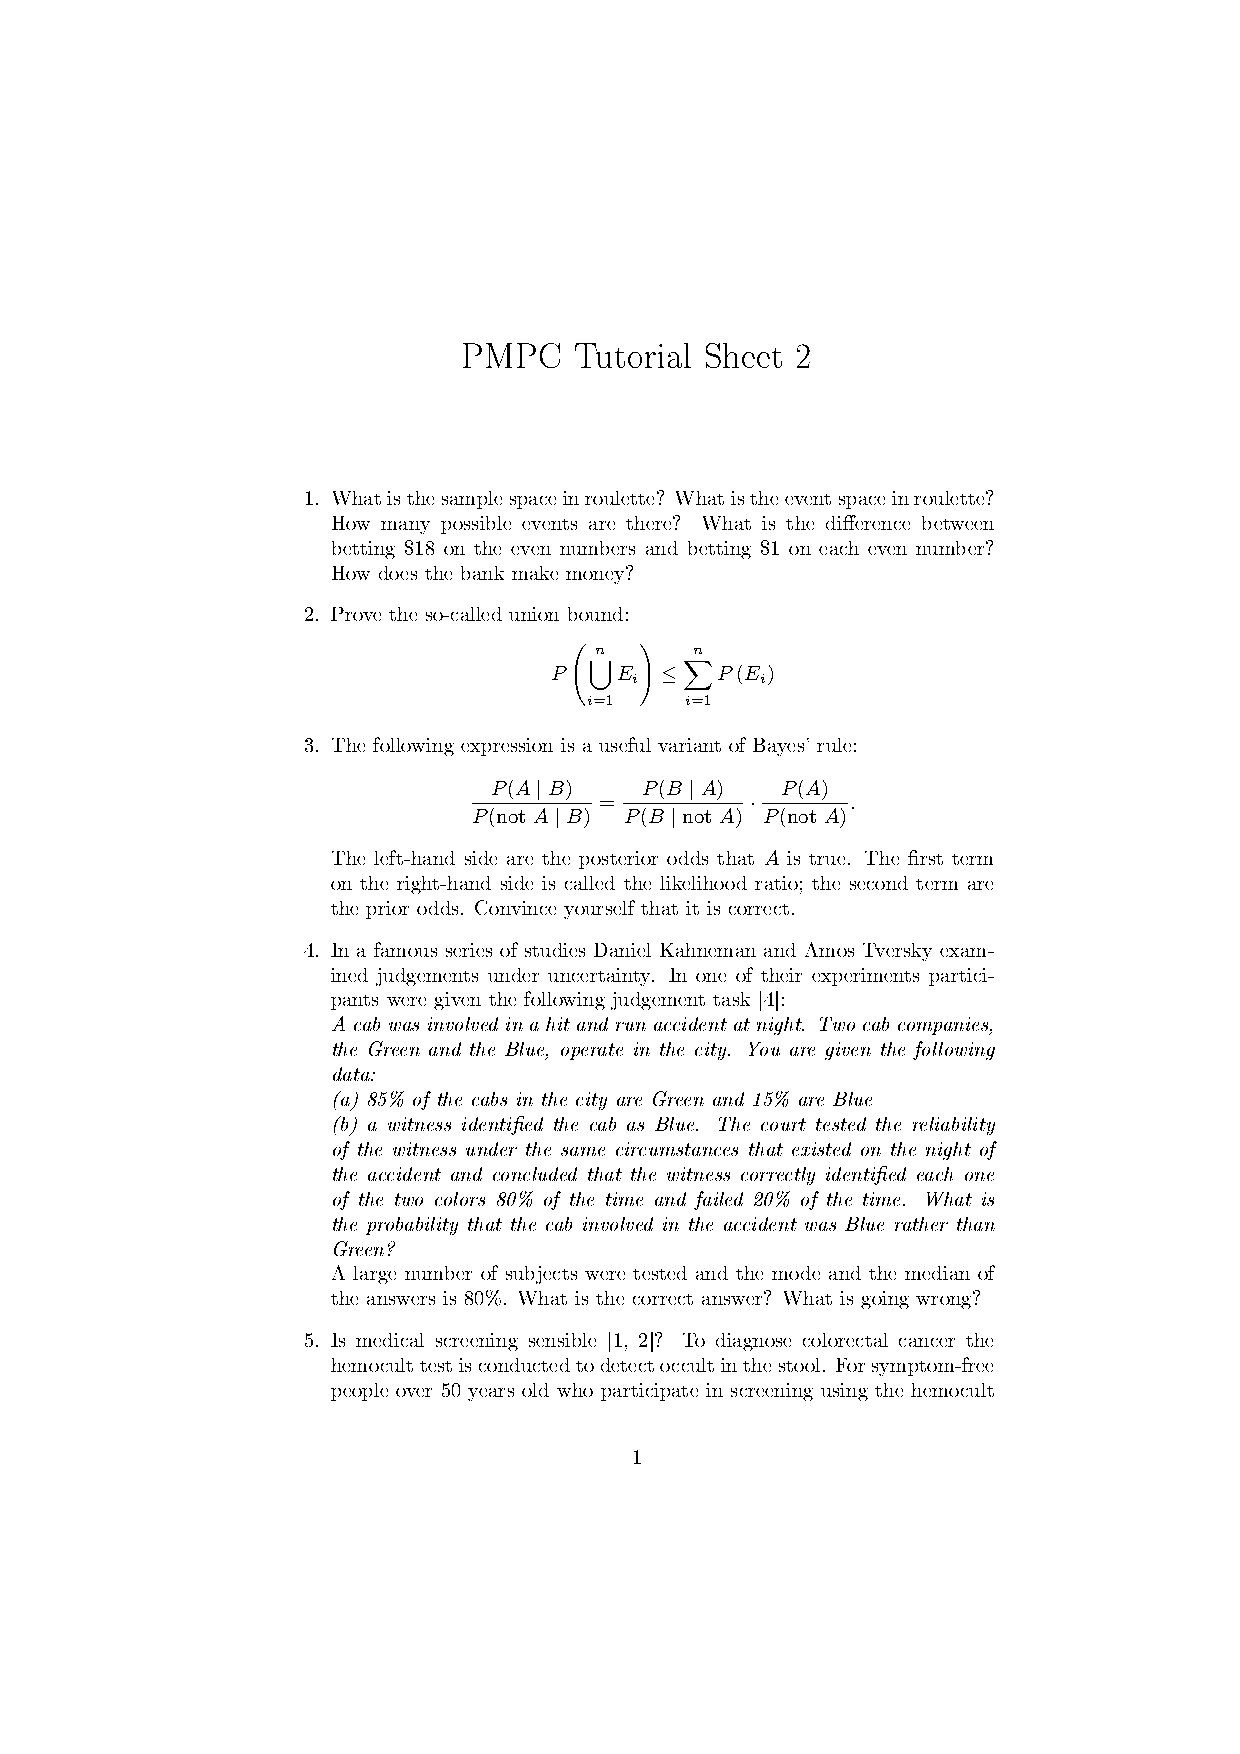
\includepdf[pages={-},
      addtotoc={1,section,1,Tutorial Sheet 2: Probability Refresher II,exsheet2},
      viewport=100 50 550 700,
      scale=0.75,
      pagecommand=\thispagestyle{plain}
      ]{../exercises/Exercises02.pdf}
}{}
\iftoggle{solutions}{
  \subfile{../chapters/2014-05-05.tex}
  \clearpage
}{}

% Measuring Beliefs I
\subfile{../chapters/2014-05-02.tex}
\clearpage

% Practice: Measuring Beliefs I
\iftoggle{exercises}{
  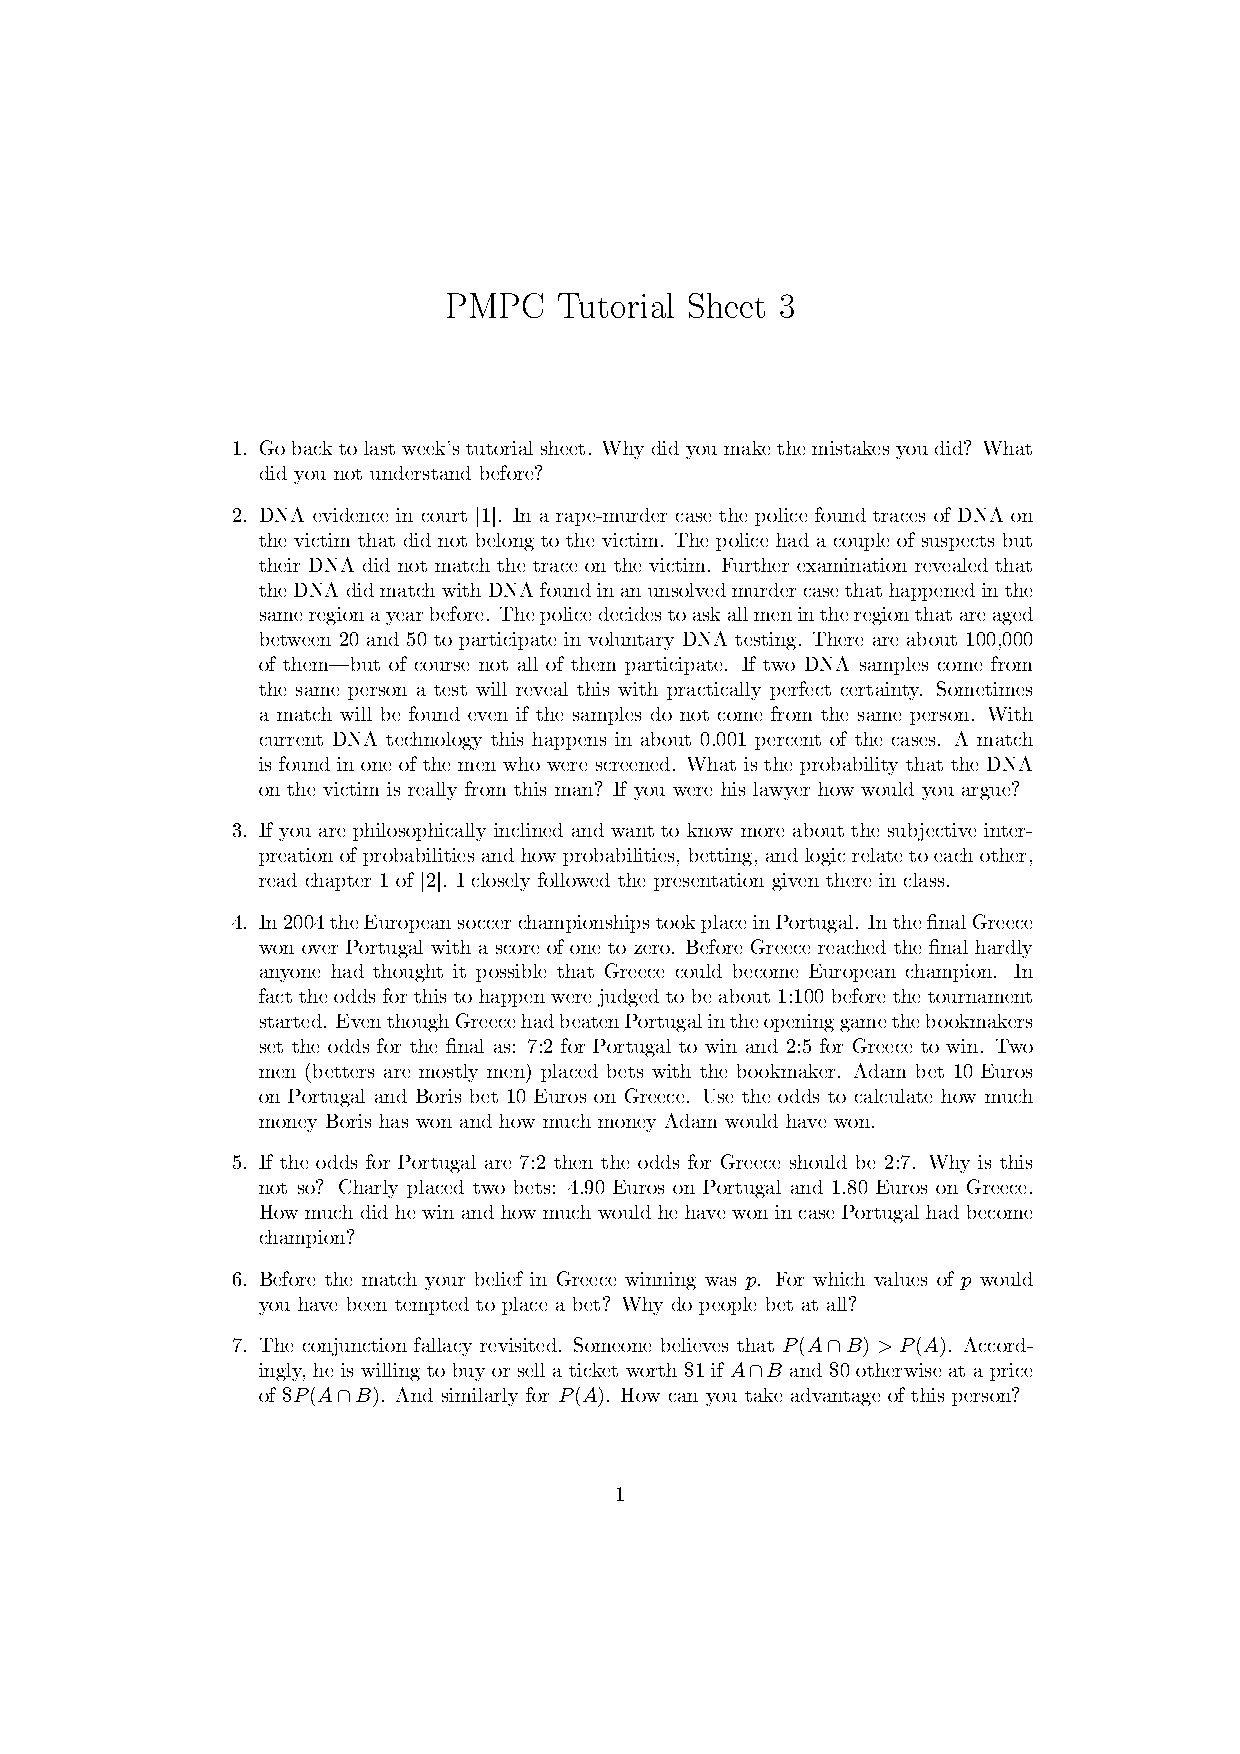
\includepdf[pages={-},
      addtotoc={1,section,1,Tutorial Sheet 3: Measuring Beliefs I,exsheet3},
      viewport=100 50 550 700,
      scale=0.75,
      pagecommand=\thispagestyle{plain}
      ]{../exercises/Exercises03.pdf}
}{}
\iftoggle{solutions}{
  \subfile{../chapters/2014-05-19.tex}
  \clearpage
}{}

% Measuring Beliefs II
\subfile{../chapters/2014-05-09.tex}
\clearpage

% Practice: Measuring Beliefs II
\iftoggle{exercises}{
  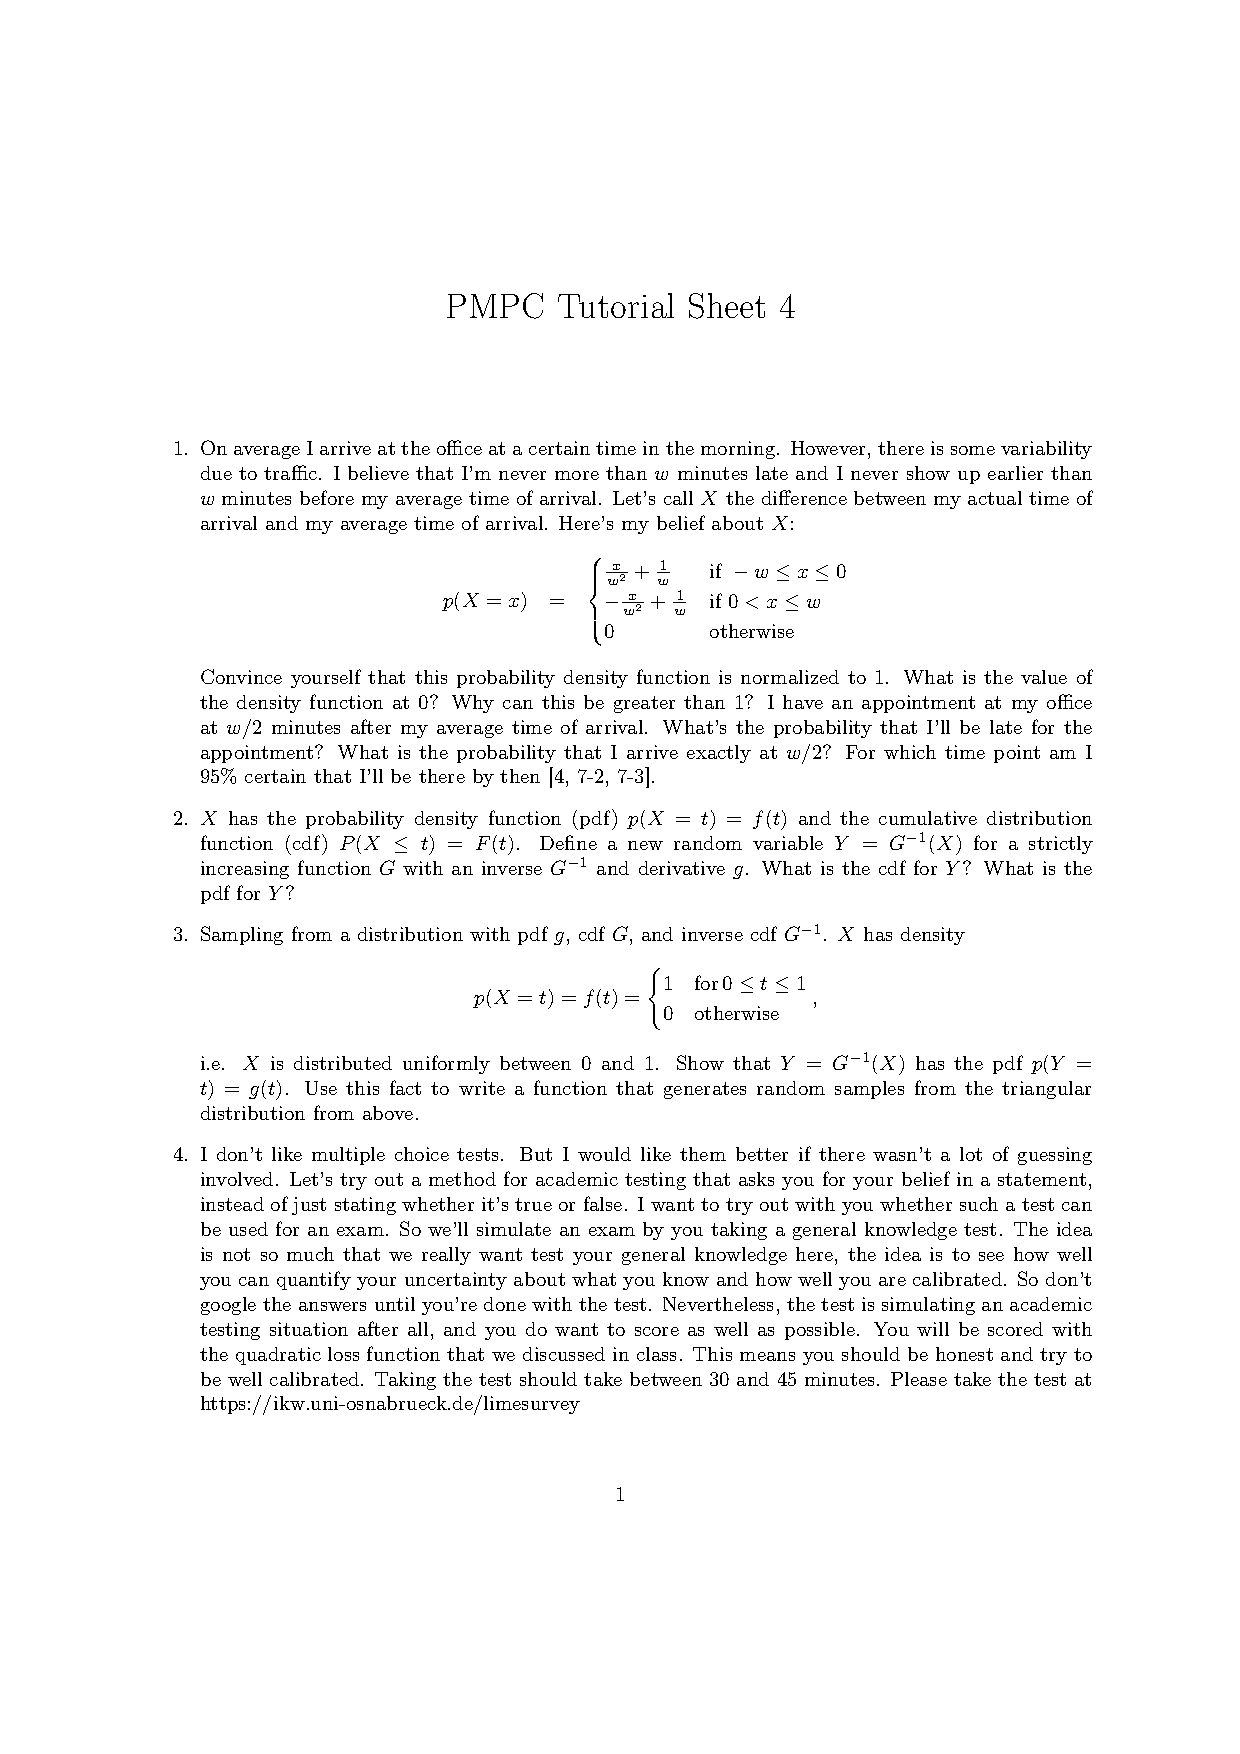
\includepdf[pages={-},
      addtotoc={1,section,1,Tutorial Sheet 4: Measuring Beliefs II,exsheet4},
      viewport=100 50 550 700,
      scale=0.75,
      pagecommand=\thispagestyle{plain}
      ]{../exercises/Exercises04.pdf}
}{}
\iftoggle{solutions}{
  \subfile{../chapters/2014-05-19b.tex}
  \clearpage
}{}

% Bayesian Inference Examples
\subfile{../chapters/2014-05-23.tex}
\clearpage

% Frequentist Inference Examples
\subfile{../chapters/2014-05-26.tex}
\clearpage

% Practice: Bayesian and Frequentist Inference
\iftoggle{exercises}{
  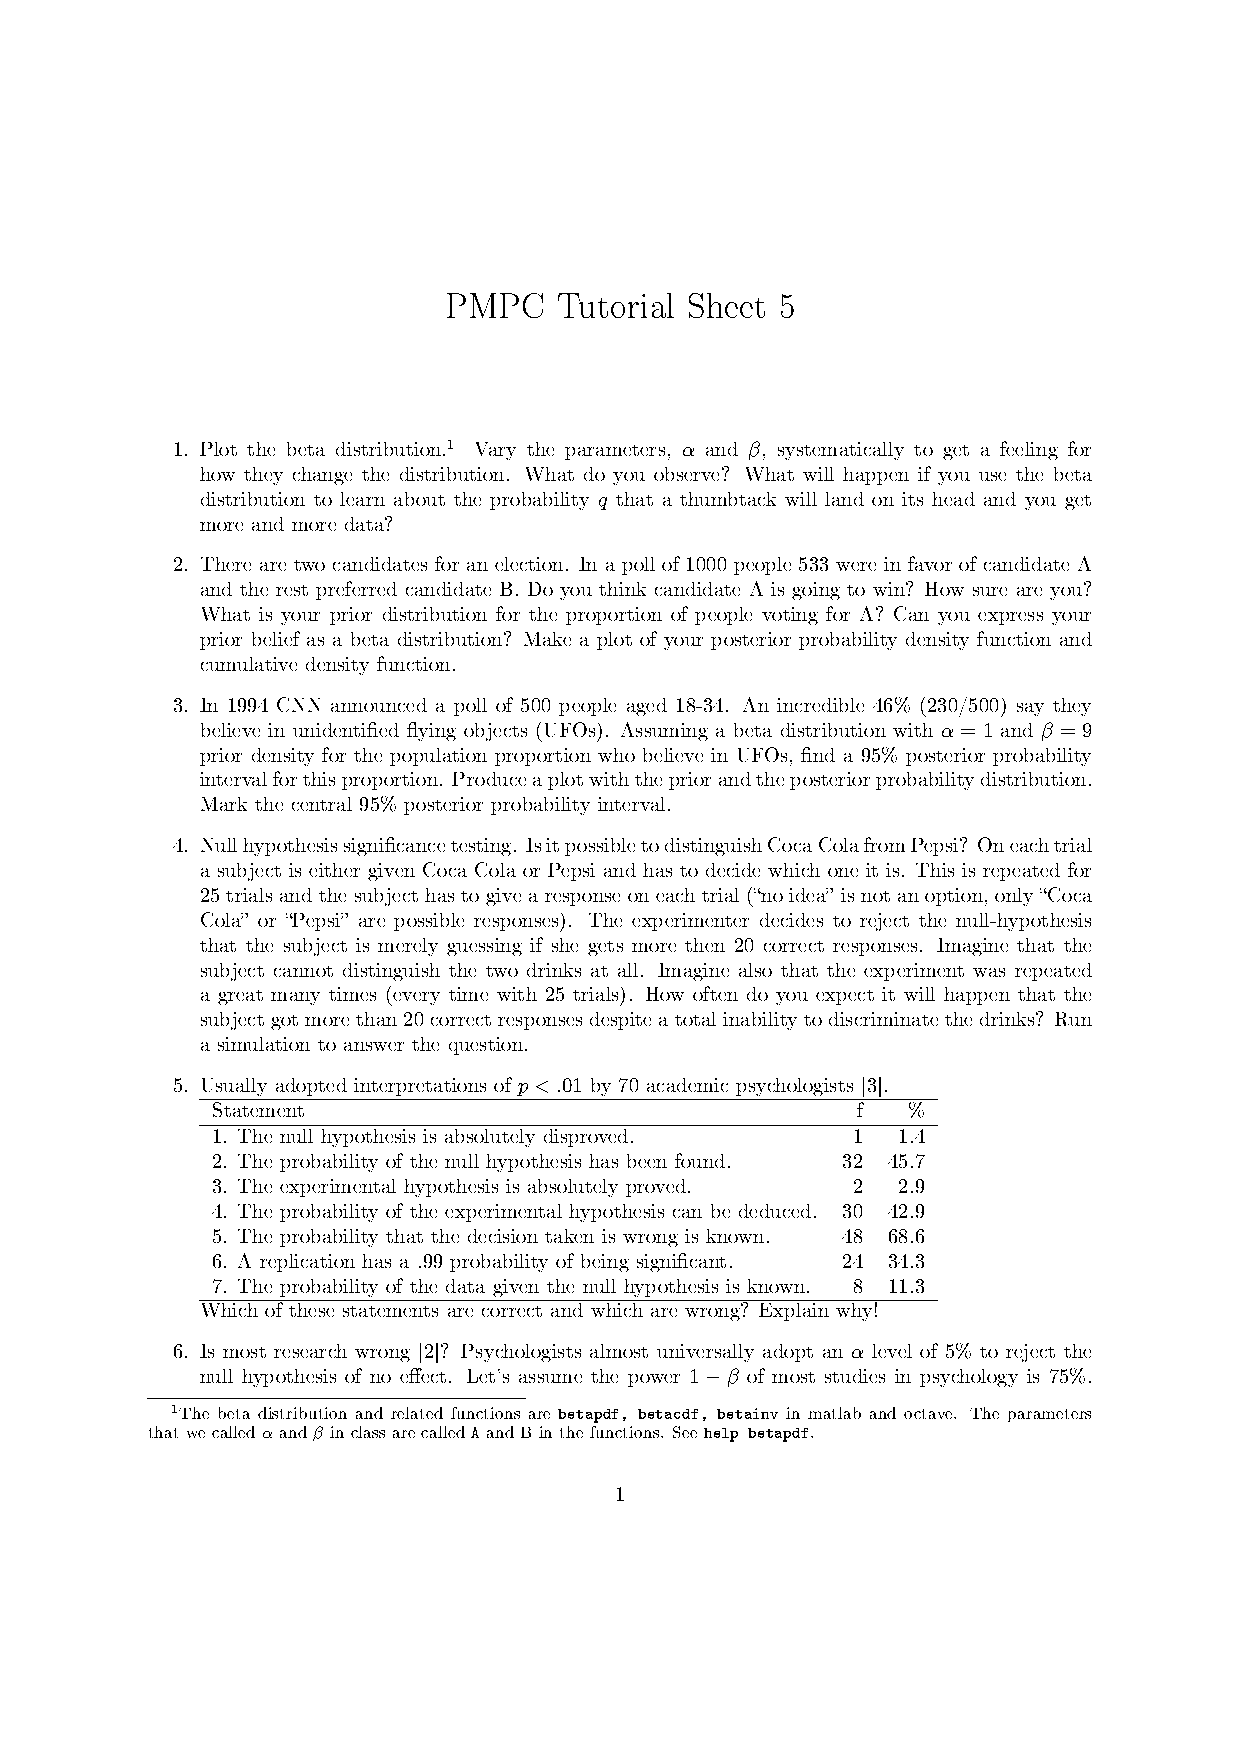
\includepdf[pages={-},
      addtotoc={1,section,1,Tutorial Sheet 5: Bayesian and Frequentist Inference I,exsheet5},
      viewport=100 50 550 700,
      scale=0.75,
      pagecommand=\thispagestyle{plain}
      ]{../exercises/Exercises05.pdf}
}{}
\iftoggle{solutions}{
  \subfile{../chapters/2014-05-30.tex}
  \clearpage
}{}

% Mid-Term exam
\iftoggle{exercises}{
  \pagestyle{plain}
  \subfile{../exercises/midterm.tex}
  \clearpage
  \pagestyle{fancy}
}{}
\iftoggle{solutions}{
  \subfile{../chapters/2014-06-06.tex}
  \clearpage
}{}

% Signal Detection Theory I
\subfile{../chapters/2014-06-13.tex}
\clearpage

% Signal Detection Theory II
\subfile{../chapters/2014-06-16.tex}
\clearpage

% Practice: Signal Detection Theory I+II
\iftoggle{exercises}{
  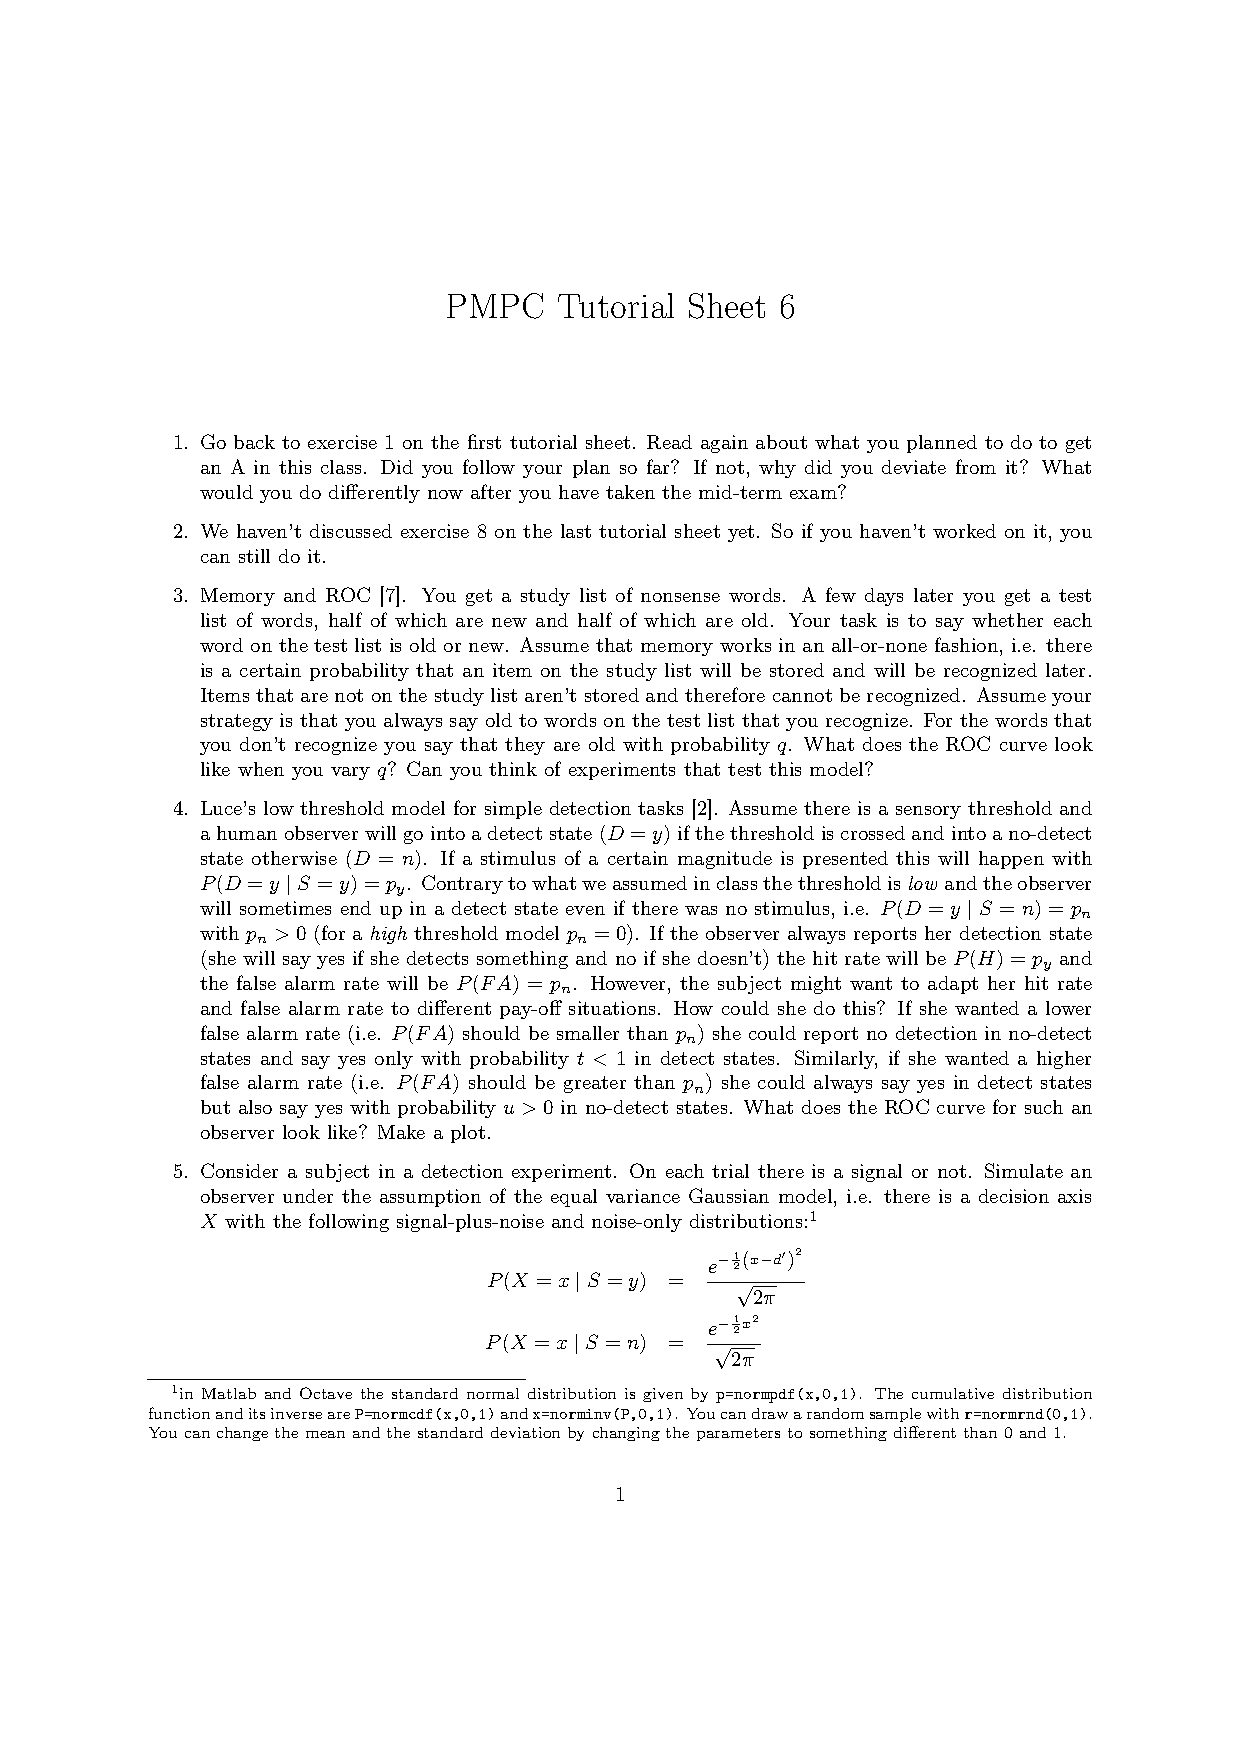
\includepdf[pages={-},
      addtotoc={1,section,1,Tutorial Sheet 6: Signal Detection Theory I+II,exsheet6},
      viewport=100 50 550 700,
      scale=0.75,
      pagecommand=\thispagestyle{plain}
      ]{../exercises/Exercises06.pdf}
}{}
\iftoggle{solutions}{
  \subfile{../chapters/2014-06-23.tex}
  \clearpage
}{}

% Signal Detection Theory III
\subfile{../chapters/2014-06-20.tex}
\clearpage

% Practice: Signal Detection Theory III
\iftoggle{exercises}{
  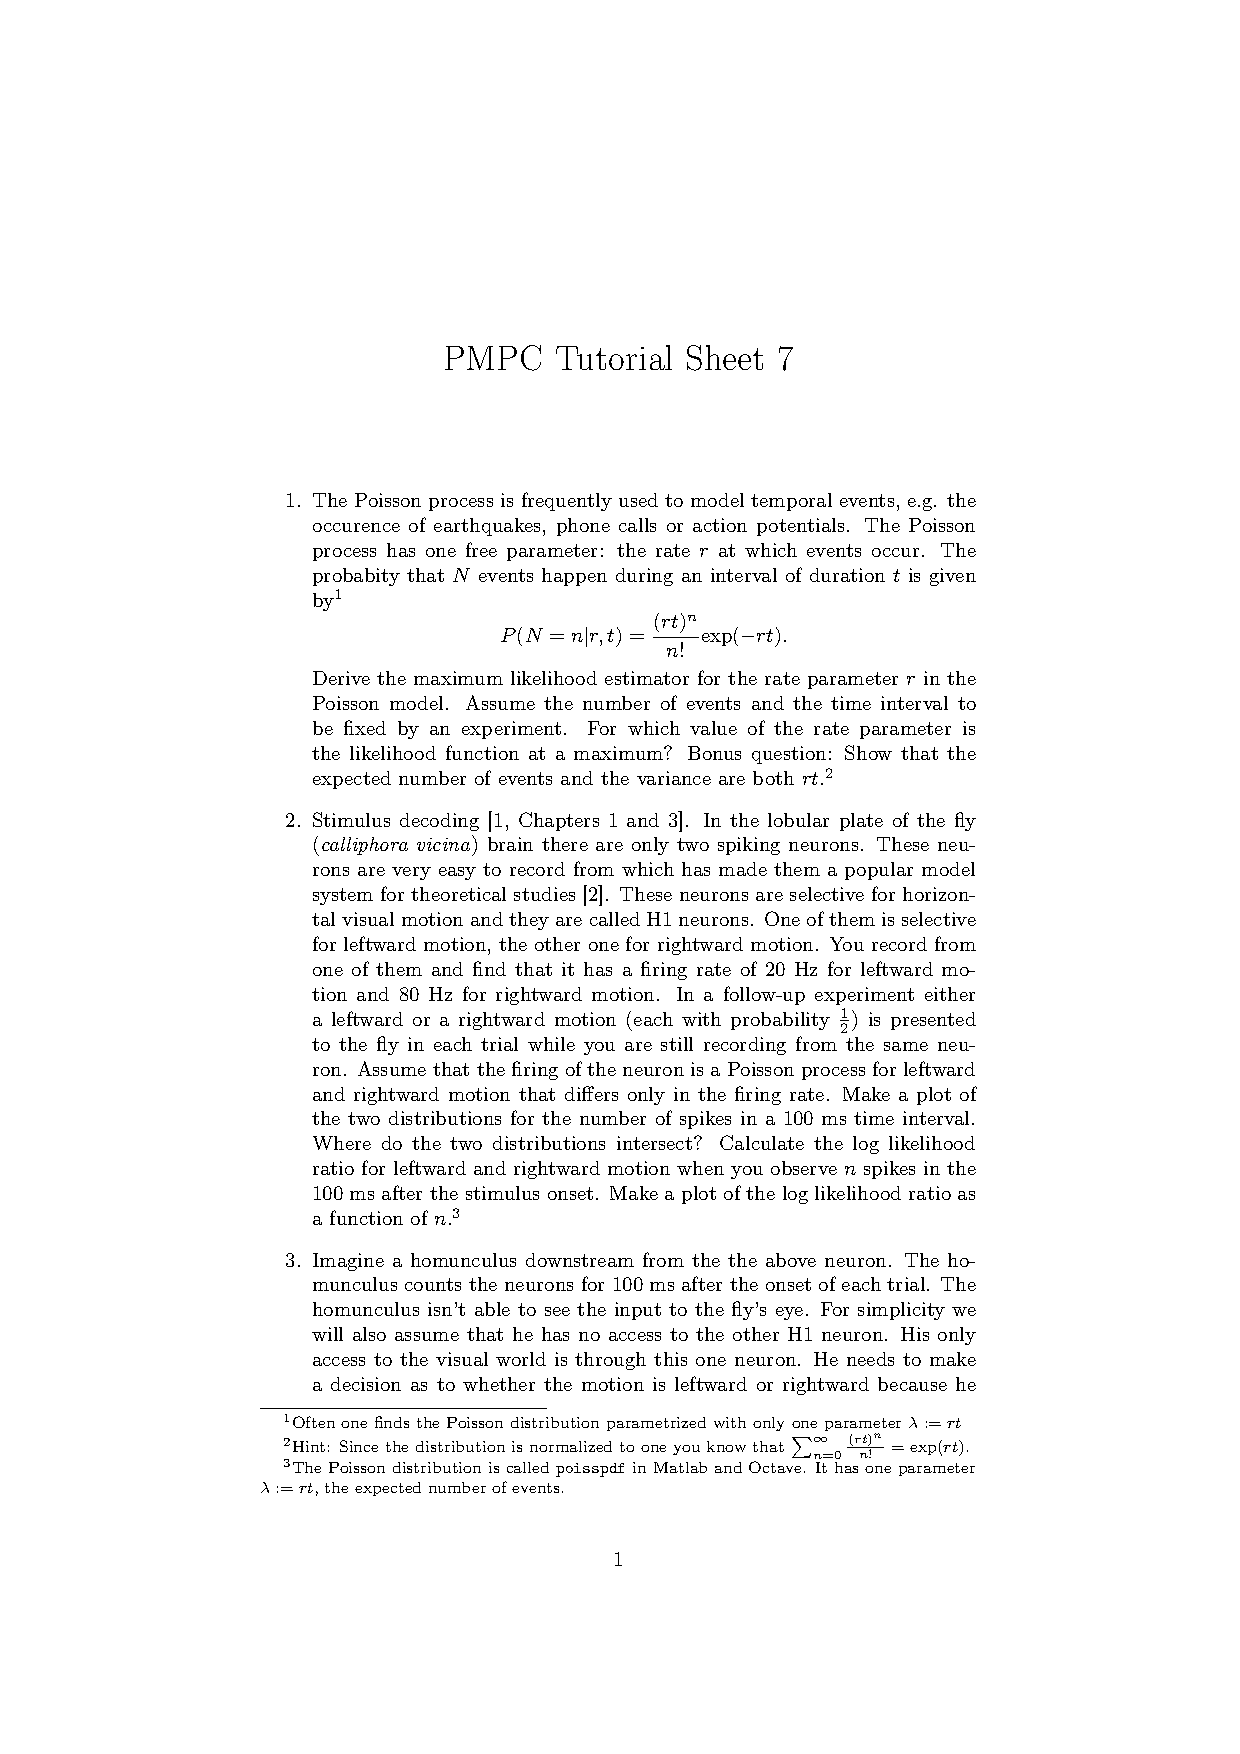
\includepdf[pages={-},
      addtotoc={1,section,1,Tutorial Sheet 7: Signal Detection Theory III,exsheet7},
      viewport=100 50 550 700,
      scale=0.75,
      pagecommand=\thispagestyle{plain}
      ]{../exercises/Exercises07.pdf}
}{}
\iftoggle{solutions}{
  \subfile{../chapters/2014-06-30.tex}
  \clearpage
}{}

% Choice Models I
%\subfile{../chapters/2014-06-27.tex}
%\clearpage

% Practice: Choice Models I
\iftoggle{exercises}{
  %\includepdf[pages={-},
      %addtotoc={1,section,1,Tutorial Sheet ,exsheet},
      %viewport=100 50 550 700,
      %scale=0.75,
      %pagecommand=\thispagestyle{plain}
      %]{../exercises/Exercises0.pdf}
}{}
\iftoggle{solutions}{
%  \subfile{../chapters/2014-07-07.tex}
%  \clearpage
}{}

% Choice Models II
%\subfile{../chapters/2014-07-04.tex}
%\clearpage

% Practice: Choice Models II
\iftoggle{exercises}{
  %\includepdf[pages={-},
      %addtotoc={1,section,1,Tutorial Sheet ,exsheet},
      %viewport=100 50 550 700,
      %scale=0.75,
      %pagecommand=\thispagestyle{plain}
      %]{../exercises/Exercises0.pdf}
}{}
\iftoggle{solutions}{
%  \subfile{../chapters/2014-07-14.tex}
%  \clearpage
}{}

% Everyday Predictions
%\subfile{../chapters/2014-07-11.tex}
%\clearpage

% Practice: Everyday Predictions
\iftoggle{exercises}{
  %\includepdf[pages={-},
      %addtotoc={1,section,1,Tutorial Sheet ,exsheet},
      %viewport=100 50 550 700,
      %scale=0.75,
      %pagecommand=\thispagestyle{plain}
      %]{../exercises/Exercises0.pdf}
}{}
\iftoggle{solutions}{
%  \subfile{../chapters/2014-07-18.tex}
%  \clearpage
}{}

% Q&A
%\subfile{../chapters/2014-07-18.tex}
%\clearpage

\clearpage
\printindex

\end{document}
